\section{Visual Encoding}
\label{sec:interface}

%We first discuss about the visual encoding of events and schemata; and then how sensemaking activities in Data-Frame model are supported in SchemaLine.
%
%\subsection{Event and Schema Representation}
%\label{sub:visual-encoding}
\subsection{Event Representation}
%Appearance
An event is represented by a rounded rectangle with its left side aligned with the event's time on the timeline. To reduce cluttering, events are not constantly connected by lines to their corresponding points on the timeline. Instead, when the mouse is over an event, its time point on the timeline is highlighted. A short textual summary is rendered inside the rectangle to summarize the event. To address the scalability of long summaries, we assign a maximum width to event rectangles and trim excess text. The full content will only be displayed when the note is hovered over. All events have a uniform height to give a consistent overall appearance, especially when they are connected to form a schema (Section \ref{sub:schema-outline}). Quite often, events are categorical data. For example, in news reports, an article can be classified into sport, fashion or both. SchemaLine adds a small rectangle in each event to color-code its categorization. Eight different colors are supported, which are chosen from qualitative colors -- Set 1 of ColorBrewer \cite{Harrower2003}. All other categories besides eight of the most popular ones will share the same color to address the limitation of the small number of distinguishable colors.\note{the other arguments we can make are that 1) we only support the most important x categories, 2) it is unlikely that more than 8 categories are displayed simultaneously} We plan to combine colors with other indicators such as texture to increase the number of differentiated keywords in the future work. The number of maximum categories that an event can belong to is configurable to adapt the dataset characteristics. As in Fig.~\ref{fig:notes-only}, maximum three themes of an event can be displayed.

\begin{figure}[ht]
\centering
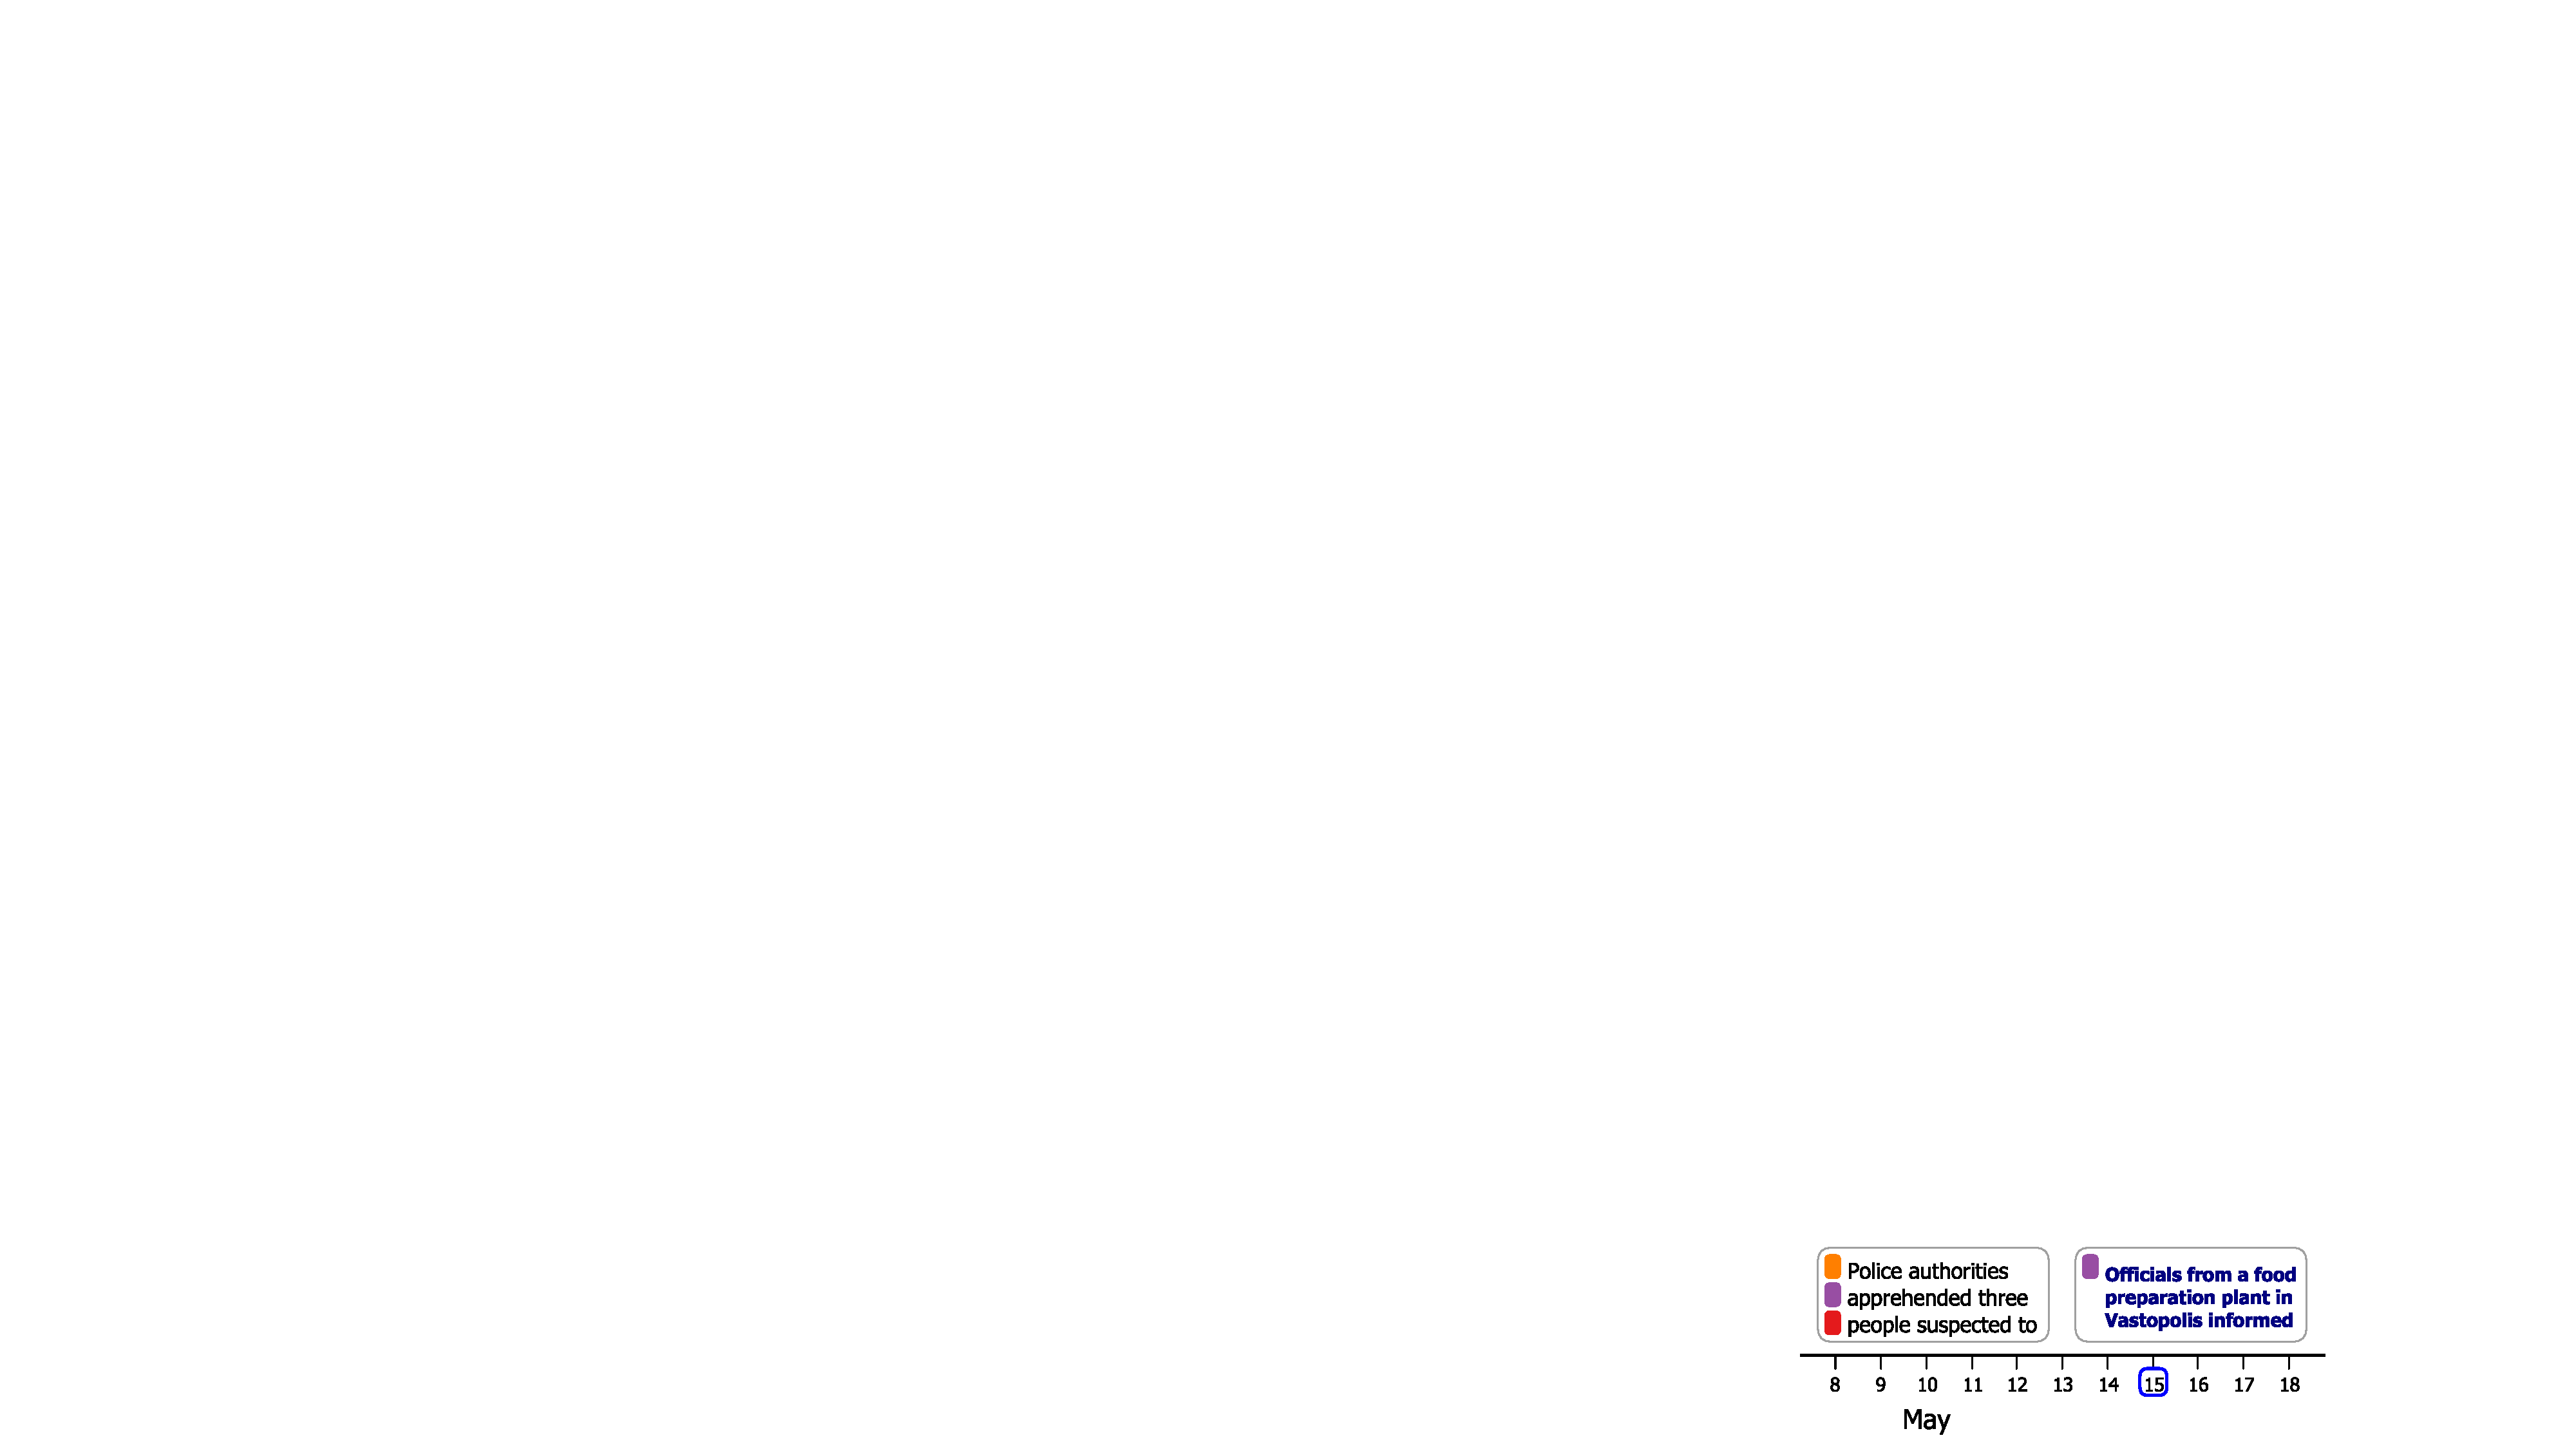
\includegraphics[width=\columnwidth]{notes-only}
\caption{Events are represented as rounded rectangles with a uniform height and limited width aligned at their corresponding time points. The 15th-May event is highlighted. On the left side of the event rectangle, small color-coded rectangles indicate the event's groupings.}
\label{fig:notes-only}
\end{figure}

%Timeline appearance
In SchemaLine, the timeline is shown as a horizontal axis at the bottom of the display. Its starting and ending points change dynamically to cover the time span of all events. The timeline consists of two temporal scales. These two scales can also be changed dynamically according to the displayed events. For example, they change from ``month/day'' to ``year/month'' to accommodate large interval increases.

\subsection{Schema Representation}
After discovering a number of relevant events or pieces of evidence, the analyst starts combining them to form a \textit{schema}. A schema is a set of related events that are connected to each other in a certain way. For example, a schema might contain all events about a particular person. Multiple schemata can be composed in SchemaLine as shown in Fig.~\ref{fig:teaser}. 

\begin{figure}[ht]
\centering
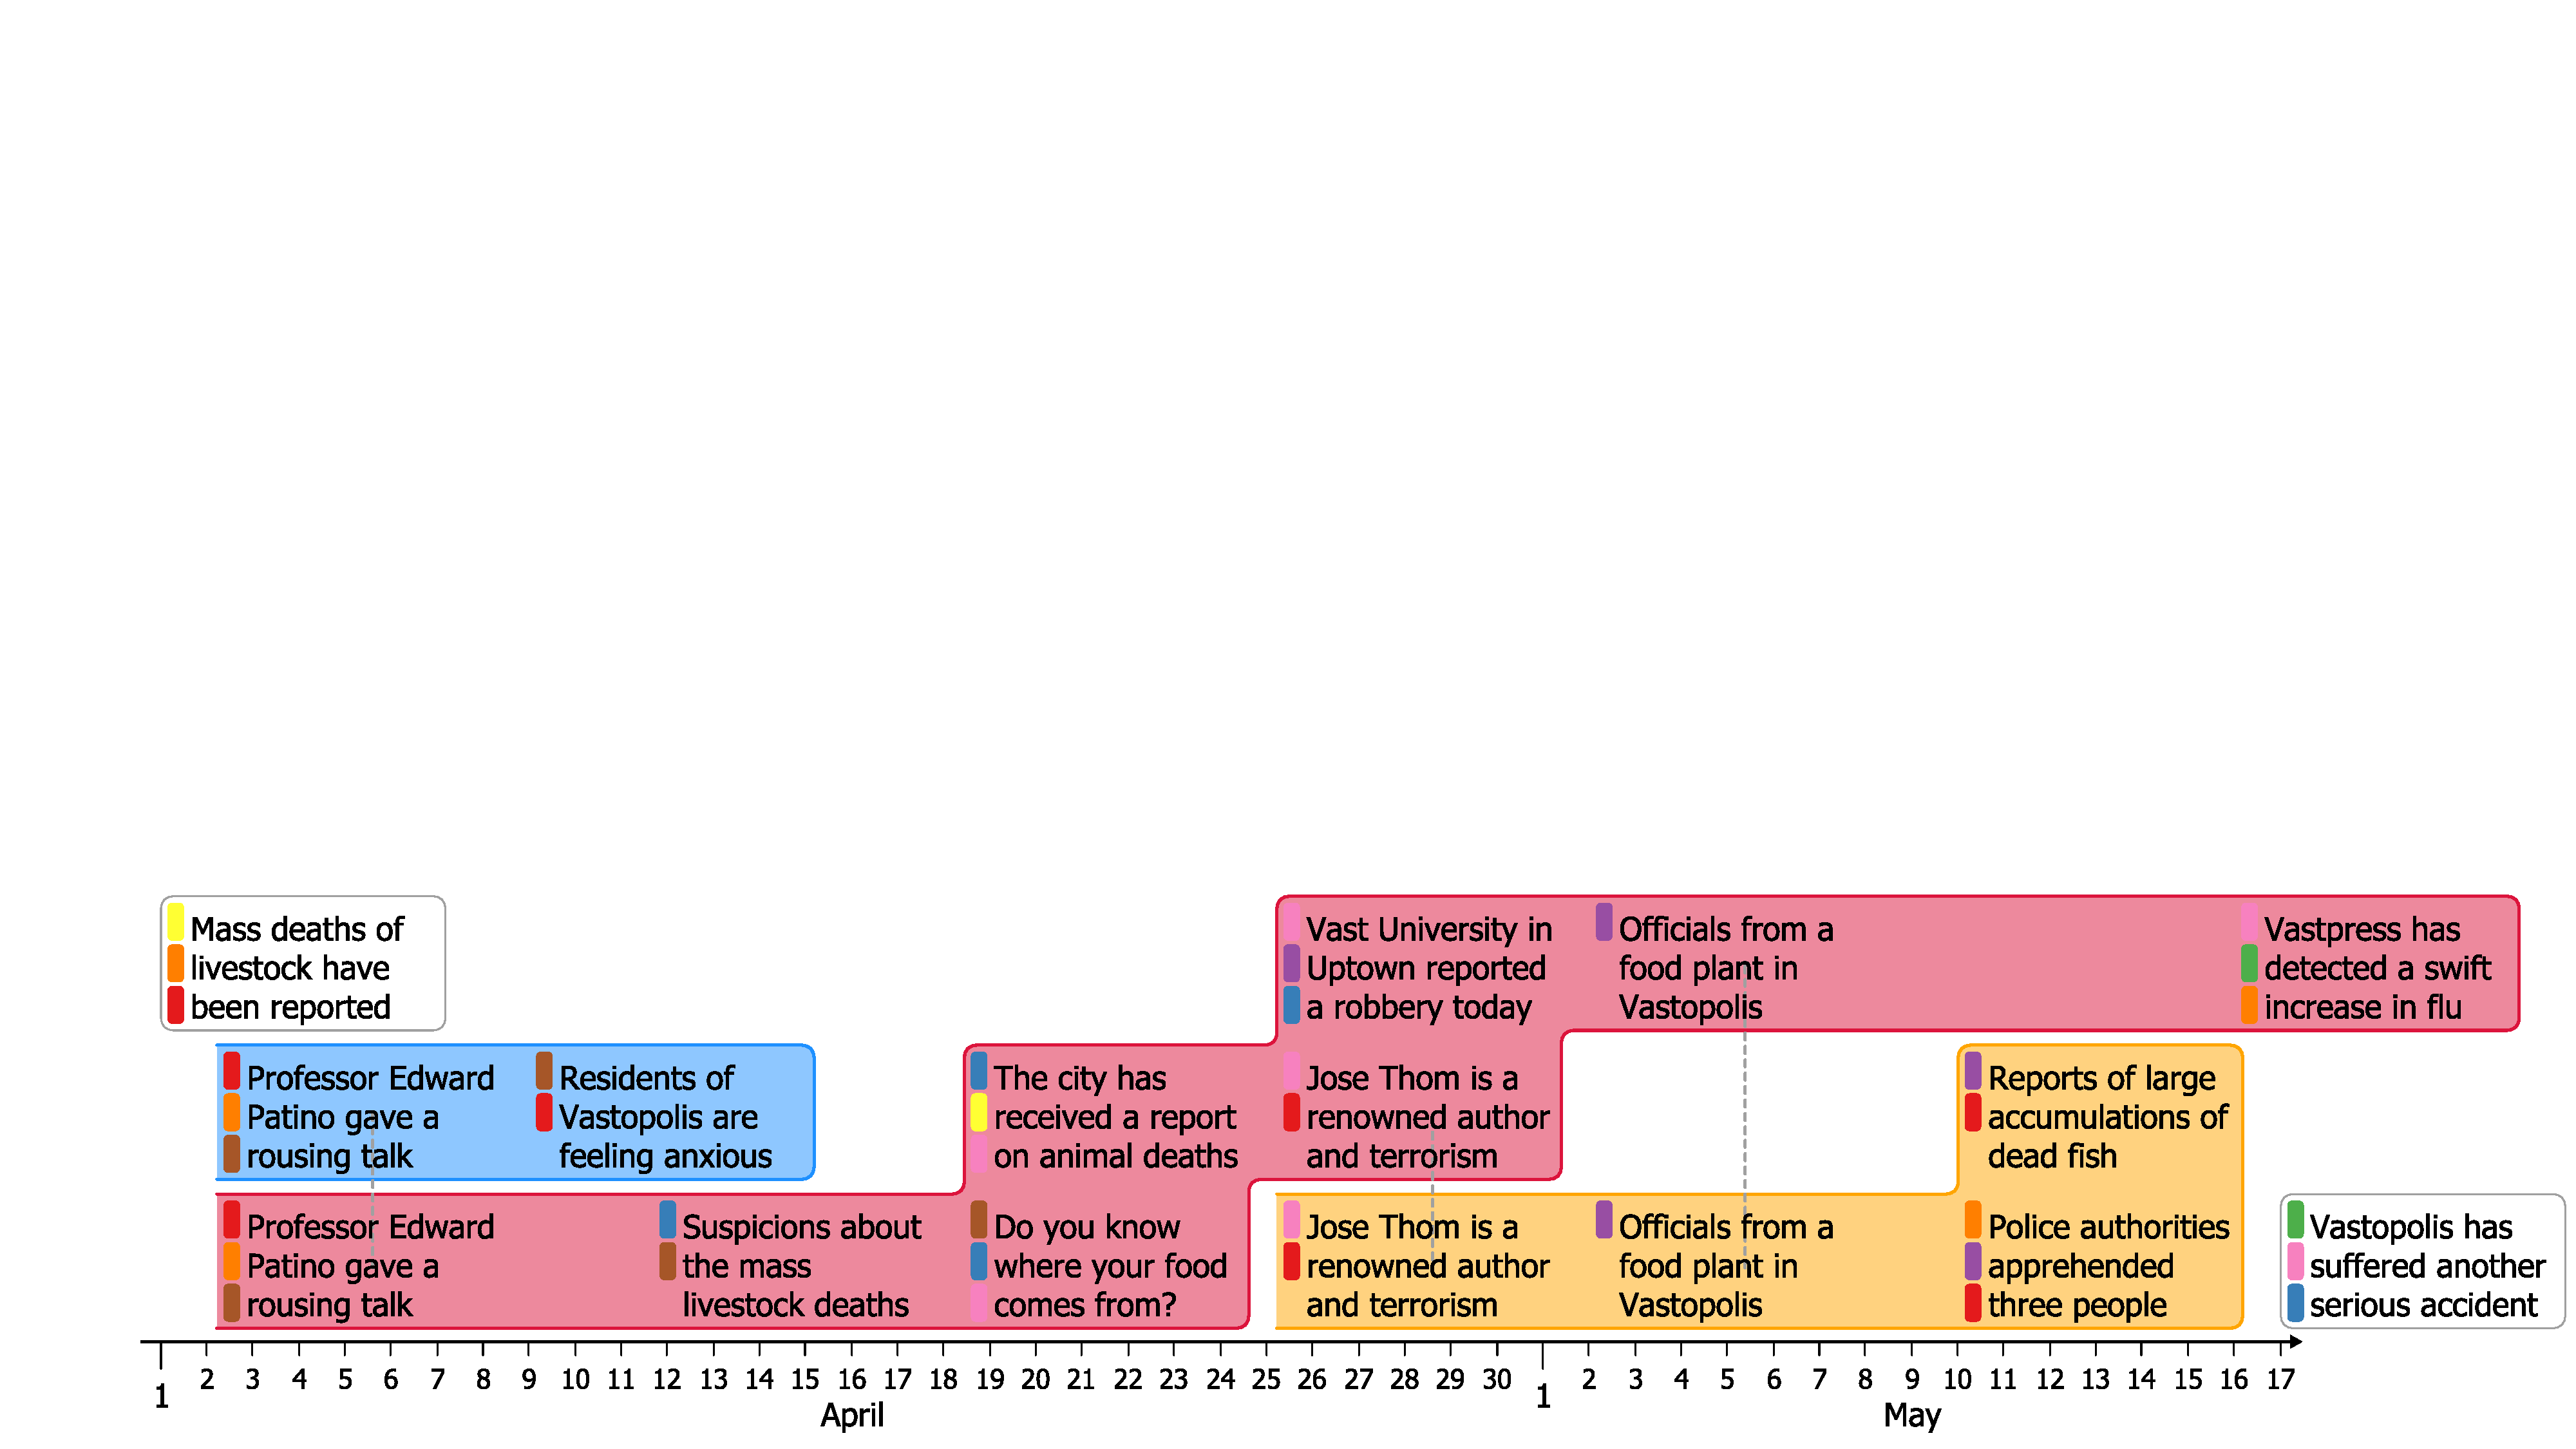
\includegraphics[width=\linewidth]{teaser}
\caption{SchemaLine: each piece of text is an analyst note, positioned along the time axis at when the event happened. Related notes are linked together to form a ``schema'' or ``frame''. There are three frames in this example represented as colored rectilinear paths. Small color-coded rectangles on the left side of notes are ``categories''.}
\label{fig:teaser}
\end{figure}

We consider several design options to connect events within a schema such as using colored/shaped icons or node-link diagrams. However, they all have some drawbacks as discussed in the Related work (Section~\ref{sec:relatedwork}). Computational methods that allow visualize a large number of events with different themes such as ThemeRiver~\cite{Havre2002} do not work either because individual events and interactions are more essential in SchemaLine. \note{I don't quite understand what the `computational' means and the argument follows} Also, it should be easy to follow events within a schema in temporal order. We decided to visualize each schema as a colored stripe, which is inspired by Munroe's hand-drawn visualization~\cite{Munroe2009}. A character line in Munroe's work connects all events happened to that character. Similarly, our schema is a color stripe connecting all events belonging to it. Instead of using a thin line, we use a path with unique width (an event's height) to make enough space to display the event's summary text and allow interaction with individual notes. A rectilinear path is employed to provide a nice visualization rather than direct connection between events. 

%In the SchemaLine, each white rectangle is an analysis note, linking to the document in the search results that led to this discovery and positioned along the time axis at the point when the event happened. Notes can be grouped together to form a ``story''. There are three stories in this example and they are in red, blue, and orange. In the middle are the results of two searches: ``vastopolis'' and ``terrorist''. At the very top is a list of minimized searches, only showing the keywords. 


%Pirolli and Card~\cite{Pirolli2005} regarded the timeline as an effective tool for the ``Schematize'' task. A timeline can not only reveal the temporal relationships among the findings, but also have a considerable impact on how easily they can be understood. Pennington and Hastie~\cite{Pennington1991} studied the impact of evidence presentation order on juror decision making. They found that information was easier to understand when presented in chronological order and thus had a significant impact on jurors' decisions. 

%\subsection{Sensemaking with Data-Frame Model}
%\label{sub:interactive-editing}
%SchemaLine is designed to support all five different sensemaking activities in Data-Frame model by fluid user interactions. Following the design guidelines for fluidity proposed by Elmqvist et al.~\cite{Elmqvist2011}, SchemaLine's interactions
%\begin{itemize}
%	\item use smooth animated transitions between states,
%	\item provide immediate visual feedback on interaction, and
%	\item use direct manipulation of visual representations.
%\end{itemize}
%
%\paragraph*{Creating a Frame}
%The first sensemaking activity in Data-Frame model is to construct a new frame by connecting relevant data. It can be achieved by dragging one event and dropping it onto another. A \textit{plus} icon and a \textit{dashed rectangle} surrounding two events are displayed to indicate that a new frame will be created. When dropping the event, a color stripe representing a schema will be formed by connecting these two events, and a smooth animated transition is used to improve user perception.
%
%\paragraph*{Elaborating a Frame}
%The analyst can elaborate the frame by adding new events to it. This activity can be performed intuitively by dragging an event, which is not a member of any frames, and dropping it onto the frame. A \textit{plus} icon is displayed to indicate the addition action will be performed. Similarly, a smooth animated transition is used to improve user perception. Fig.~\ref{fig:drag-drop-note} shows an example of adding an event into a frame.
%\begin{figure}[ht]
%\centering
%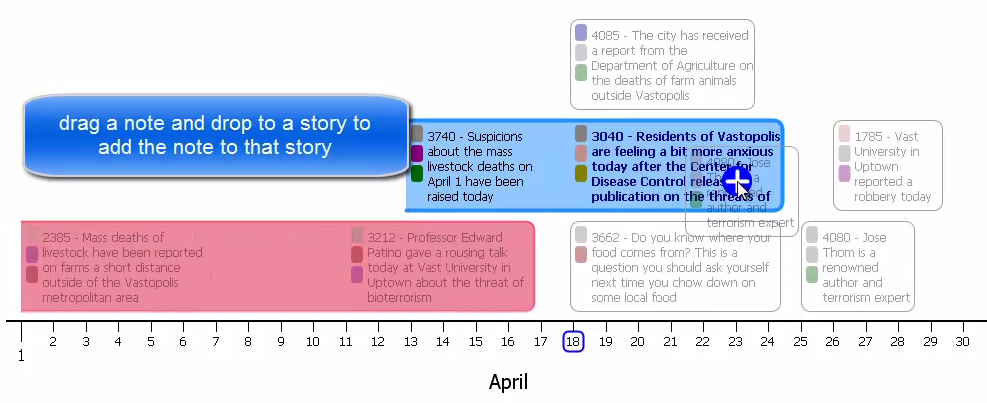
\includegraphics[width=\linewidth]{drag-drop-note}
%\caption{Each schema is represented as a colored stripe. Dropping an event onto the blue stripe means adding that event into the blue schema.}
%\label{fig:drag-drop-note}
%\end{figure}
%
%\paragraph*{Questioning a Frame}
%Visual encoding of the event's themes may help detect inconsistencies in data within a frame. The temporal distribution of events among the schema may suggest some concerns about the validity or completeness of the frame. For example, if a frame about one person contains many events in January and March, but no events are found in February. It may be inferred that there should be some data missing. The analyst can mark a suspected event by right-mouse double-clicking on it. Red color text is used to indicate that the event needs more investigation. 
%
%\paragraph*{Preserving a Frame}
%The first possible action when encountering inconsistent data is to discard the data and preserve the frame. The analyst remove an event from the frame by dragging it outside the frame and dropping it onto the void space. A \textit{minus} icon is displayed to indicate the subtraction action will be performed. A smooth animated transition is also used to improve user perception. Right-mouse double-clicking onto a suspected event to flip its status back to normality.
%
%\paragraph*{Reframing}
%The second possible action to handle inconsistent data is to modify the frame itself.
%SchemaLine supports that one event can belong to multiple frames. This allows the analyst to create several similar frames and compare them. Holding \textit{Control} key when dropping a note onto a frame will create a duplicate event. The analyst can also move an event from one frame to another by simple drag-and-drop interaction.
%
%\subsection{Events-Only Interactions}
%Other interactions with events are also designed to be intuitive to avoid menus or buttons wherever possible. Left-mouse double-clicking on to an event is to open its full content. Dragging an event with mouse right-click can change the event's date. This feature is useful because the report date is not always the date when the event actually happens. Also, dragging an event outside the boundary of the timeline will remove it from the system (with \textit{remove} icon as an informative feedback).
%
%Once any change is made on SchemaLine, such as moving an event from one schema to another, an animation is made to produce a smooth transition between the changes to help analyst update their ``mental map''. To achieve that, event rectangles are interpolated between the old and the new locations. The schema outline algorithm (Section \ref{sub:schema-outline}) runs at every step of the interpolation to produce intermediate polygon paths based on the updated event location.